La biogéographie est l'étude de la répartition géographique des espèces.
Aujourd'hui, dans un monde où les écosystèmes sont très perturbés, les
biogéographes comptent parmi leurs missions celle d'établir des
scénarios de changement de la biodiversité. Cependant, les efforts de
recherche accumulés sur plus d'un siècle ont révélés des obstacles
majeurs à la compréhension de l'action simultanée des mécanismes
dessinant les aires de distribution des espèces, faisant de la
prédictions de ces distribution un véritable défi. En réponse à ces
difficultés, certains auteurs ont proposés d'aller vers un
renouvellement de la théorie de la discipline. Parmi les étapes majeures
de ce renouvellement figure l'intégration des interactions écologiques
au sein d'une théorie plus intégrative de la biogéographie. C'est
justement sur ce point qu'ont porté mes travaux de thèse. J'ai
particulièrement réfléchi sur comment intégrer les interactions dans des
modèles de distribution d'espèces, c'est-à-dire envisager le reflet des
liens écologiques qui nouent les espèces entre-elles dans la géométrie
de leur répartition géographique.

Je propose dans la présente introduction de cerner un peu mieux les
enjeux de ma thèse. Pour cela, je commence par montrer que la
compréhension des mécanismes déterminant la distribution des espèces
était très avancée dès la fin du XIX\textsuperscript{ème} siècle durant
lequel, après plus de 150 ans de voyages d'exploration scientifique, la
connaissance plus exhaustive de la richesse biologique terrestre a mené
à la théorie de l'évolution. Je souligne que dès les années 1960, la
biogéographie s'est dotée d'une théorie ambitieuse qui a grandement
participé à la compréhension de l'ensemble des processus mis en jeu. Je
présente ensuite différents cadres conceptuels en biogéographie qui,
bien que présentant de nombreuses qualités sont aujourd'hui appelés à
intégrer davantage de processus écologiques, comme les interactions
écologiques. Je reviens dans un dernier temps plus en détails sur ce
point pour contextualiser l'objet central de ma thèse qui a donné des
éléments de réponse à deux grandes questions~: comment intégrer les
interactions écologiques dans des modèles en biogéographie? Quelles
traces ces interactions laissent-elles sur la géométrie des aires de
répartition?

\section*{Des îles et des espèces}\label{des-uxeeles-et-des-espuxe8ces}
\addcontentsline{toc}{section}{Des îles et des espèces}

\subsection*{En suivant Wallace}\label{en-suivant-wallace}
\addcontentsline{toc}{subsection}{En suivant Wallace}

Dans l'introduction de son livre \emph{Island Life} paru en 1881, le
célèbre naturaliste Alfred Russel Wallace nous rapporte deux faits
étonnants qui justifient pleinement l'examen attentif de la répartition
géographique des espèces \citep{wallace1881island}. Premièrement, le
biogéographe démontre, à l'aide de nombreux exemples, que l'éloignement
entre deux régions du monde n'est pas suffisant pour conclure quant à
l'éloignement de leur composition faunistique et floristique. Ainsi, la
comparaison des avifaunes de l'île japonaise d'Hokkaido et de
l'Angleterre, séparées par des milliers de kilomètres, révèle une
proximité des paysages ornithologiques très supérieure à celle constatée
dans l'analyse comparée des oiseaux des îles indonésiennes de Bali et de
Lombok pourtant distantes de quelques kilomètres seulement.
Deuxièmement, en s'appuyant sur les différences des faunes brésilienne
et africaine, Wallace souligne la faiblesse du pouvoir prédictif des
variables climatiques pour décrire les compositions faunistiques
présentes sous des latitudes similaires. Ces constatations soulignent
l'utilité de croiser les informations des distributions à la lumière
d'une analyse taxonomique pour y apporter du sens. Dans le cadre de la
théorie de l'évolution\footnote{Wallace a publié en 1858 un article
  \emph{On the Tendency of Varieties to Depart Indefinitely From the
  Original Type} qui témoigne très clairement que ses idées sur les
  variations temporelles des espèces qui étaient très proches de celles
  de Charles Darwin à qui il avait d'ailleurs envoyé son manuscrit avant
  que \emph{De l'origine des espèces} ne soit publié
  \citep{Wallace1858}.}, encore toute jeune en 1881, cette analyse
taxonomique est une analyse historique~: Wallace montre que la
compréhension d'un problème spatial, celui des aires de répartition de
groupes d'espèces, n'est possible que par une compréhension temporelle,
celle de l'histoire des espèces. Cette idée est clairement énoncée dans
la suite de son introduction~:

\begin{quote}
Many years study of this class of subjects has convinced me that there
is no short and easy method of dealing with them; because they are, in
their very nature, the visible outcome and residual product of the whole
past history of the earth.
\end{quote}

Tout au long de son livre, Wallace démontre que la connaissance à
l'échelle mondiale de la distribution des êtres vivants permet
d'associer les différentes îles aux grands ensembles régionaux
biologiques (que nous appelons aujourd'hui écozones) sur la base des
ressemblances biologiques des espèces qui témoignent du lien temporel
unissant les différentes zones géographiques de la Terre. Ce travail de
caractérisation d'ensembles géographiques conduit notamment Wallace,
dans un article de 1860 \citep{Wallace1860}, à tracer la ligne éponyme
séparant l'écozone indomalaise de l'écozone australienne (séparant les
îles de Bali et Lombok mentionnée au paragraphe précédent). La
connaissance apportée à la géographie par l'histoire est saisissante et
les exemples de Wallace deviennent autant d'arguments en faveur de la
théorie de l'évolution. Le discours de Wallace porte sur des processus à
des échelles spatiales et temporelles très grandes\footnote{L'âge de la
  terre est très débattu à l'époque. Bien que l'ensemble des savants
  s'accordent pour aller bien au-delà des 6000 ans bibliques, il n'y a
  alors pas de consensus. Wallace affirme à la page 212 du chapitre 10
  de \emph{Island Life} que la vie se développait il y a au moins 500
  millions d'années \citep{wallace1881island}, ce qui est audacieux pour
  l'époque mais bien en-dessous de l'âge des plus anciens fossiles
  découverts à ce jour qui a estimé en 2011 à 3.4 milliards d'années
  \citep{Wacey2011}.}, ce qui apporte un éclairage substantiel qui se
double cependant d'un obstacle épistémologique majeur~: si l'explication
ultime de la présence d'une espèce en un point donné est le produit
d'une série de contingences historiques, quelles peuvent être les
fondations d'une théorie de la biogéographie? Ce n'est qu'au
XX\textsuperscript{ème} siècle que des réponses convaincantes
émergeront.

\subsection*{En suivant MacArthur et
Wilson}\label{en-suivant-macarthur-et-wilson}
\addcontentsline{toc}{subsection}{En suivant MacArthur et Wilson}

Parmi les visions les plus importantes de la biogéographie, figure celle
contenue dans le livre publié en 1967 \emph{The Theory of Island
Biogeography}, produit de la fructueuse rencontre du mathématicien et
biologiste Robert MacArthur et du myrmécologue Edward Wilson\footnote{Cet
  actuel professeur émérite à l'université d'Harvard est reconnu pour
  ses apports en biologie et en sociologie, il est notamment l'auteur de
  32 livres. C'est pour son immense connaissance des fourmis que j'ai
  choisi le nom de myrmécologue.}. À partir d'un grand nombre de données
sur les faunes insulaires de diverses régions du monde, ces auteurs ont
construit un cadre théorique élégant pour expliquer les variations du
nombre d'espèces sur ces îles \citep{MacArthur1967}. Leur démarche
théorique permet de lier des observations à un modèle mathématique
donnant une explication simple et convaincante des variations étudiées.
Ils font ainsi basculer la discipline dans une ère nouvelle, ce dont les
auteurs étaient conscients, comme en atteste le premier paragraphe du
dernier chapitre de leur livre~:

\begin{quote}
Biogeography has long remained in a natural history phase, accumulating
information about the distribution of species and higher taxa and the
taxonomic composition of biotas. Interpretative reasoning has been
largely directed to the solution of special problems connected with the
histories of individuals taxa and biotas. Without doubt this descriptive
activity will continue to be of fundamental importance to the science,
one of the most physically adventurous of all scientific entreprises
and, in the richness of the detail it unfolds, esthetically pleasing.
But biogeography is also in a position to enter an equally interesting
experimental and theoretical phase.
\end{quote}

Dans cet extrait, MacArthur et Wilson affirment que l'étude de la
distribution des espèces doit sortir du royaume des contingences
historiques pour devenir un objet de science au sens d'être manipulé
aussi bien expérimentalement que par l'abstraction mathématique. La
validation expérimentale de la théorie a d'ailleurs été menée par Wilson
et son étudiant au doctorat de l'époque, Daniel Simberloff, devenu
depuis un écologue reconnu \citep{Simberloff1969}. Le travail
d'abstraction mathématique a été conduit par MacArthur dans le livre de
1967 et prolongé dans les annexes de son livre de 1972
\citep{macarthur1972geographical}. Ces auteurs proposent une explication
de la variation spécifique des îles fondée sur deux processus opposés~:
la colonisation d'espèce depuis le continent qui augmente le nombre
d'espèces sur l'île et un processus d'extinction locale qui diminue ce
nombre. C'est en reliant ces processus aux propriétés physiques de l'île
(aire et isolation) et en interprétant la richesse spécifique des îles
en terme d'équilibre entre ces deux processus que les auteurs
parviennent à expliquer de manière convaincante les relations observées
entre richesse spécifique, taille de l'île et isolement. Dans le
troisième temps de cette introduction, je reviens amplement sur cette
théorie nommée théorie de la biogéographie des îles que je noterai TIB
(pour \emph{Theory of Island Biogeography}) dans la suite.

Le paradigme de la TIB est un lègue qui a eu un impact considérable sur
les développements théoriques en écologie \citep{Warren2015}. Au centre
du projet de la TIB, se loge la volonté de mettre l'espèce au coeur de
la biogéographie afin de permettre à la discipline de s'enrichir des
mécanismes biologiques qui sont un moteur essentiel de la variation dans
la distribution des espèces. L'intérêt de leur » biogéographie de
l'espèce » \citep[le terme est mentionné à l'avant-dernière phrase de
l'ouvrage][p.183]{MacArthur1967} est dans l'affirmation qu'il faut
regarder les contraintes conjointes de l'évolution (qui met un certain
nombre d'espèces avec des caractéristiques propres en présence) et du
contexte écologique qui détermine les conditions de colonisation et
d'extinction. Cette intrication de l'écologie et de l'évolution est bien
inscrite dans la pensée de MacArthur et Wilson même si la puissance de
leur vision réside dans le fait de les occulter en partie.

Près de 50 ans après la parution de leur livre, une des clefs en
biologie semble être la compréhension des rétroactions qu'il existe
entre écologie et évolution dans les variations spatiales et temporelles
de la biodiversité. Je reprends ici trois aphorismes cités par
\citet{Schoener2011a} concernant les liens entre biologie, écologie et
évolution~: « Nothing in biology makes sense except in the light of
evolution. » \citep{Dobzhansky1973}; « Nothing in evolutionary biology
makes sense except in the light of ecology. » \citep{grant2008}; «
Nothing in evolution or ecology makes sense except in the light of the
other. » \citep{Pelletier2009a}; La chronologie de ces citations est un
indice de la reconnaissance actuelle du besoin (de la nécessité?) de
croiser écologie et évolution. Un parallèle avec les sciences humaines
me semble possible dans lequel l'écologie serait à la biologie ce que la
géographie est aux sciences humaines et l'évolution serait à la biologie
ce que l'histoire est aux sciences humaines. Nous pouvons certes étudier
l'une sans l'autre, mais le dialogue entre les deux disciplines est
indispensable afin d'éviter que chacune avancent en faisant des
hypothèses fortes sur l'autre qui finiront éventuellement par nuire à
une compréhension plus profonde de la biologie. Par exemple, supposer
que les variations démographiques ont des origines purement écologiques
devient problématique si les variations génétiques sont suffisantes pour
expliquer qu'une partie importante de cette variation comme cela l'a été
montré sur une population de moutons de Soay \citep{Pelletier2007}. Je
ne cherche pas à nier l'utilité des savoirs acquis de manière autonome
par un champ disciplinaire, j'insiste simplement sur l'importance de
mettre ces connaissances en perspective les unes avec les autres en vue
d'une synthèse indispensable pour décrypter l'information contenue dans
les distributions d'espèces.

\subsection*{Quelles informations renferment les distributions
d'espèces?}\label{quelles-informations-renferment-les-distributions-despuxe8ces}
\addcontentsline{toc}{subsection}{Quelles informations renferment les
distributions d'espèces?}

Cette question est non seulement une invitation à découvrir les raisons
de la présence de tel ou tel organisme en un lieu donné du globe, mais
elle suggère aussi que certaines informations ne peuvent pas être
obtenues par la seule analyse de la répartition géographique des
espèces. Les auteurs mentionnés dans les paragraphes précédents y ont
apporté des éléments de réponse cruciaux~: Wallace a montré que les
distributions géographiques reflétaient en partie les liens de parenté
entre les espèces, quant à MacArthur et Wilson, ils ont suggéré que ces
distributions étaient le résultat de processus écologiques dynamiques.
Examiner les aires de répartition, en détailler la géométrie exacte et
les variations spatio-temporelles, faire des recoupements entre les
répartitions géographiques de différentes espèces ou encore avec la
distribution de variables abiotiques sont des démarches fondamentales
pour en apprécier les mécanismes sous-jacents.

Dans son ouvrage de 1972, MacArthur discute de l'ensemble de ces
mécanismes, il considère aussi bien le rôle que peuvent jouer les
variables climatiques que celui des interactions écologiques. En plus
des exemples concrets amenés pour illustrer ses propos, MacArthur
développe des modèles mathématiques pour prolonger la discussion. Dans
son second chapitre, il formalise l'impact de la compétition sur la
coexistence des espèces aboutissant ainsi sur un principe de ségrégation
spatiale des espèces liées par ce type de relation~: deux compétiteurs
ne peuvent pas co-occurrer (résider durablement au même endroit) sauf
éventuellement sur une zone très restreinte de leur distribution
\citep{macarthur1972geographical}. Toujours dans cet ouvrage, MacArthur
évoque la distribution en damier (\emph{checkerboard}) que peuvent
générer des espèces en compétition. La discussion de ce type de
distribution sera approfondie par Jared Diamond \citep{Diamond1975} dont
les travaux déclencheront un débat important sur la détermination de
modèles nuls de co-occurrence \citep{Connor1979} et sur laquelle mon
travail de thèse apporte quelques éléments nouveaux.

L'étude des limites spatiales d'un grand nombre d'espèces permet d'y
déceler des généralités quant aux mécanismes qui les déterminent
\citep{macarthur1972geographical}. L'examen des variations
spatio-temporelles apporte une information très utile sur l'importance
relative des divers mécanismes. Le contexte des changements climatiques
est une bonne illustration de ce principe car les bouleversements
actuels des répartitions géographiques des espèces permettent en effet
de pointer le rôle majeur des mécanismes micro-évolutifs auparavant
sous-estimés \citep{Lavergne2010}. Enfin, l'examen des distributions
doit aussi être un examen des co-distributions~: il faut s'intéresser à
l'information de sous-ensembles d'espèces et notamment aux espèces en
interaction afin de tester si la biologie laisse des empreintes dans la
géométrie des aires de répartition. Par exemple, dans mes travaux de
thèse, je propose de regarder l'intersection de l'aire associée à un
ensemble de proies pour savoir ce qu'elle nous apprend sur la
distribution de leur prédateur (présenté au chapitre \ref{chap3}).

\subsection*{Enjeux de la connaissance de la répartition géographique
des
espèces}\label{enjeux-de-la-connaissance-de-la-ruxe9partition-guxe9ographique-des-espuxe8ces}
\addcontentsline{toc}{subsection}{Enjeux de la connaissance de la
répartition géographique des espèces}

Les observations et la compréhension des causes profondes de la
géométrie et la dynamique des aires de répartitions des espèces ont déjà
mené à des découvertes majeures en écologie et en évolution. La phase
d'expérimentation et de théorisation de la biogéographie décrite par
MacArthur et Wilson se poursuit et se tourne vers un objectif très
ambitieux~: faire de la biogéographie une discipline prédictive,
pourvoyeuse de prédictions fiables sur les aires de répartitions futures
de n'importe quelle espèce \citep{Mouquet2015, Warren2015}. Ce problème
est d'autant plus présent dans la littérature récente que nous sommes
dans un contexte où ces aires sont profondément bouleversées. En
biogéographie, les changements climatiques ont en effet canalisé
l'attention des chercheurs qui constatent avec stupeur l'ampleur à
laquelle la biodiversité mondiale est affectée
\citep{Koh2004, Bellard2012}. La volonté d'anticiper la localisation
future des espèces a également engendré des efforts conséquents pour
développer des outils statistiques essentiellement centrés sur la
corrélation entre les variables abiotiques et les données de présence
(d'occurrence) des espèces \citep{Elith2006}.

En ciblant l'étude de la distribution de certaines espèces, la
biogéographie rencontre des enjeux socio-économiques majeurs. Ainsi,
pour un pays comme la France, la restriction des zones favorables à la
croissance de la vigne envisagée à l'aide des scénarios de changements
climatique \citep{Hannah2013} pourrait conduire à des pertes économiques
importantes et un bouleversement identitaire des grandes régions
viticoles. De plus, détecter aujourd'hui un potentiel viticole futur
dans des régions où cette production n'existe pas peut conduire à des
augmentations drastiques du prix des terres agricoles. En guise de
second exemple, je pose la question suivante~: où seront les érablières
de demain? La réponse est donnée par la détermination de la répartition
future des aires favorables à la croissance de l'érable à sucre
(\emph{Acer saccharum}) et à sa capacité à les atteindre afin de s'y
établir \citep{Solarik2016}.

Je termine avec un troisième exemple~: la perte des pollinisateurs et
notamment des abeilles. Pas moins de quatre grandes classes de facteurs
d'origine anthropique les mettent en danger~: les changements
climatiques, le changement dans l'utilisation des terres\footnote{Parmi
  les changements les plus problématiques relatifs aux terres agricoles
  figurent la monoculture et l'utilisation massive de pesticides. Les
  pesticides de la famille des néonicotinoïdes semblent affaiblir les
  colonies d'abeilles.}, l'apparition de nouveaux pathogènes (dont
l'acarien parasite \emph{Varroa destructoa} vecteur de nombreux virus)
et l'arrivée d'espèces invasives \citep[comme le frelon
asiatique][]{Vanbergen2013}. Le défi actuel est de prédire la
distribution future des pollinisateurs en intégrant ces multiples
aspects et leurs interactions. De plus, dans le cas des espèces
invasives, il faut comprendre comment une espèce peut sortir de son aire
de répartition naturelle et en établir une nouvelle.

Actuellement, les outils de prédiction des aires de répartition futures
reposent essentiellement sur les scénarios de changements climatiques
\citep{Peterson2011}. Ces modèles dits de distribution d'espèces (que je
noterai SDMs dans la suite en référence au terme anglais \emph{Species
Distribution Models}) proposent une démarche cohérente~: la connaissance
basée sur les corrélations de variables climatiques permet d'établir une
relation climat-répartition d'espèce. En utilisant les résultats des
climatologues qui dérivent les variations climatiques associées à des
scénarios d'émission de gaz à effet de serre par les activités humaines,
les biogéographes établissent les probabilités de présence des espèces
dans les conditions climatiques futures. Cependant, la relation
climat-présence n'est qu'une facette du lien qui unit les espèces à
l'espace et chaque nouvelle invasion nous montre à quel point il est
difficile de prédire les aires de répartitions. Ces problèmes de qualité
des prédictions sont le reflet de lacunes théoriques qui amènent
plusieurs chercheurs à se positionner en faveur d'un renouvellement des
fondations théoriques pour édifier une biogéographie plus intégrative
\citep{Lomolino2000, Beck2012, Thuiller2013}. Bien sur, ces appels
soulèvent des défis importants dont on ne peut qu'espérer qu'ils soient
relevés au plus vite pour faire face à la crise environnementale
actuelle.

\subsection*{Travail théorique et
modélisation}\label{travail-thuxe9orique-et-moduxe9lisation}
\addcontentsline{toc}{subsection}{Travail théorique et modélisation}

Avant d'énumérer, avec des exemples concrets, l'ensemble des forces qui
régissent la répartition géographique d'une espèce, je souligne dans
cette partie l'importance du travail de théorisation et de modélisation
qui joue un rôle prépondérant dans mes travaux de doctorat.

\subsubsection*{Rassembler et intégrer des
faits}\label{rassembler-et-intuxe9grer-des-faits}
\addcontentsline{toc}{subsubsection}{Rassembler et intégrer des faits}

Le travail de théorisation est avant tout la mise en cohésion d'un
certain nombre de faits, d'observations. Dans la TIB, par exemple,
MacArthur et Wilson proposent une explication cohérente de
l'augmentation de la richesse spécifique dans les îles de plus grande
taille. De manière générale et poppérienne, trois principes encadrent la
construction d'une théorie scientifique~:\\
1. la théorie doit pouvoir être testée (par une expérience ou par la
récolte de données),\\
2. la théorie doit être falsifiable~: la théorie demeure valide tant
qu'elle n'est pas prouvée fausse, tant qu'une théorie alternative ne la
supplante pas,\\
3. la théorie doit être parcimonieuse, ne pas invoquer de multiples
processus sans raison (c'est-à-dire sans une augmentation du nombre de
faits expliqués), c'est un principe qui est aussi connu sous le nom de
Rasoir d'Ockham.

Une boutade, dont je suis malheureusement incapable de me souvenir de
l'auteur, énonce que les physiciens expliquent 95\% de l'univers avec 5
règles alors que les économistes expliquent 5\% des phénomènes qu'ils
étudient avec 95 règles\footnote{Une variante indique que les
  économistes ont prédit douze des trois dernières crises économiques.
  Je pense que pour ce qui est de nos capacités de prédictions, la
  biogéographie est plus proche de l'économie que de la physique.}. Le
problème n'est pas tant de dénigrer une discipline mais de constater
d'un côté la puissance prédictive d'une théorie mature et de l'autre,
les problèmes posés par une théorie lacunaire. En biogéographie, j'ai le
sentiment que les théories manquent de maturité; la TIB donne certes une
vision cohérente de la richesse spécifique insulaire mais c'est une
théorie peu précise~: prédire un nombre d'espèces n'aide que
partiellement à comprendre le monde qui nous entoure. Pour faire un peu
de prospective, une théorie qui donnerait des prédictions sur la
composition des réseaux insulaires plutôt que sur la richesse spécifique
supplanterait la TIB car elle expliquerait davantage de faits au prix
probable d'une complexité supérieure.

\subsubsection*{Des modèles pour explorer et tester la
théorie}\label{des-moduxe8les-pour-explorer-et-tester-la-thuxe9orie}
\addcontentsline{toc}{subsubsection}{Des modèles pour explorer et tester
la théorie}

Le terme de modèle signifie simplement que l'objet en question a des
propriétés bien connues. Un organisme modèle, par exemple, est un
organisme souvent facile à élever et manipuler, et pour lequel beaucoup
de connaissances ont été acquises; il sert souvent d'unité empirique
pour un ou plusieurs groupes de recherche. Les modèles statistiques sont
des outils pour tester des relations basées sur des hypothèses issues de
théories. De même, pour un travail de modélisation mathématique, la
description du modèle est contenue dans une série d'équations dérivées
d'une théorie et de savoirs empiriques. À travers les modèles, quelle
qu'en soit leur nature, on explore et on teste une théorie que l'on a
éventuellement participé à établir.

Les modèles sont souvent décrits comme une simplification de la
réalité~: comment, en effet, prétendre que les mécanismes biologiques
décelés chez \emph{Arabidopsis thaliana}\footnote{Il s'agit de la plante
  modèle par excellence dont le génome fut le premier à être séquencé
  chez les plantes \citep{TheArabidopsisGenomeInitiative2000}.} sont les
mêmes que ceux à l'œuvre pour l'ensemble des plantes à fleurs? Pour
combien de systèmes proie-prédateur le modèle de Lotka-Volterra est-il
pertinent? Les limites des modèles doivent être reconnues, mais il ne
faut pas nier l'apport de ces derniers. Les modèles sont autant
d'occasions pour explorer une ou plusieurs prédictions d'une théorie. Le
choix du modèle employé est lié à l'histoire du chercheur qui l'utilise,
à ses propensions à utiliser avec succès telle ou telle démarche
scientifique, c'est ce que rappelle Kevin McCann dans la préface de son
livre \emph{Food Webs} \citep{mccann2011food} :« It just so happens that
some people find it easier to think about things in terms of x's and
y's, and other in terms of rabbits and lynx. » En d'autres termes,
certaines personnes ont plus de facilités pour penser en termes
d'abstractions mathématiques alors que d'autres font meilleur usage de
représentations plus concrètes. Je me réclame volontiers de la première
catégorie de personnes, je pense que les mathématiques fournissent un
cadre de pensée très puissant, comme l'indique le célèbre écologue
Robert May \citep[ p.~791]{May2004}~:

\begin{quote}
The virtue of mathematics in such a context is that it forces clarity
and precision upon the conjecture, thus enabling meaningful comparison
between the consequences of basic assumptions and the empirical facts.
Here mathematics is seen in its quintessence: no more, but no less, than
a way to think clearly.
\end{quote}

Dans mes travaux, j'ai essayé d'utiliser les mathématiques pour
développer des modèles dont le point de départ a été une réflexion
collective autour du rôle que pouvaient jouer les interactions dans la
répartition géographique des espèces. J'ai alors établi un cadre
théorique avec lequel j'ai dérivé des prédictions dont certaines
semblent être vérifiées dans les données empiriques.

\subsubsection*{Nouvelles prédictions}\label{nouvelles-pruxe9dictions}
\addcontentsline{toc}{subsubsection}{Nouvelles prédictions}

Après l'établissement d'une théorie expliquant un certain nombre de
faits et pour laquelle un certain nombre de tests ont été réalisés, le
raisonnement fondé sur celle-ci peut conduire à la production de
nouvelles prédictions dont la vérification la renforceront. En revanche,
l'apparition de faits expérimentaux en désaccord avec cette théorie
demanderont des réponses qui se traduiront soit par une meilleure
compréhension de la limite d'application de la théorie soit par
l'émergence d'une théorie nouvelle qui expliquera ces faits nouveaux
tout en couvrant le rayon de compréhension de la théorie précédente
\citep{Popper1959}. Ces dernières années, la physique nous a donné deux
exemples très probants du pouvoir de l'imagination doublé du cadre
rigoureux des mathématiques avec la vérification expérimentale de
théories énoncées bien avant que les outils permettant de la vérifier
existent. En 2012, c'est la détection du Boson de Higgs dont l'existence
fut prédite en 1964\footnote{Pour plus de détail, je renvoie le lecteur
  au bulletin du CERN disponible en ligne
  \url{http://cds.cern.ch/journal/CERNBulletin/2012/28/News\%20Articles/1459456?ln=fr}}.
Cette année, c'est la détection des ondes gravitationnelles 100 ans
après qu'Albert Einstein en ait prédit l'existence \citep{Waldrop2016}.
En biogéographie, une théorie devrait être capable, par exemple, de
dresser des cartes de potentiel d'invasion à l'échelle mondiale pour
l'ensemble des espèces. Je pense que nous en sommes encore loin,
néanmoins, le chemin pour y parvenir passe par une connaissance
approfondie de l'ensemble des mécanismes qui interviennent dans le tracé
des aires de répartition, c'est-à-dire connaître leur nature, leur
portée mais aussi leurs interactions et leurs importances relatives.

\section*{Les processus qui façonnent les aires de
répartition}\label{les-processus-qui-fauxe7onnent-les-aires-de-ruxe9partition}
\addcontentsline{toc}{section}{Les processus qui façonnent les aires de
répartition}

\subsection*{Biogéographie
historique}\label{bioguxe9ographie-historique}
\addcontentsline{toc}{subsection}{Biogéographie historique}

Il s'agit de la compréhension des impacts sur les êtres vivants des
événements de grande amplitude temporelle (allant de quelques milliers
d'années à plusieurs millions d'années). C'est dans l'étude de la
proximité des taxons et des fossiles découverts que l'on peut déchiffrer
les mouvements de colonisation des différentes branches de l'arbre du
vivant. Pour prendre l'exemple d'un phénomène de très grande amplitude,
on peut faire appel à la théorie de la dérive des continents établie par
Alfred L. Wegener\footnote{La similarité des fossiles trouvés sur des
  continents très éloignés a été un des arguments en faveur de cette
  théorie.} qui implique que des groupes éventuellement proches il y a
des millions d'années ont été séparés et ont donné naissance à des
lignées différentes. Aujourd'hui, nous sommes capables de retracer ces
liens de parenté à l'aide de phylogénies moléculaires qui sont des
outils très efficaces pour estimer le temps que sépare différentes
espèces. Ainsi, par la comparaison des génomes mitochondriaux, il a été
montré récemment que les lémuriens (primates malgaches) ont été séparées
de toute autre lignée de primates il y a 60 millions d'année environs
\citep{Finstermeier2013}. Cette séparation questionne la série
d'événements qui ont conduit à l'isolation de ce groupe de singes à
Madagascar et à la construction des communautés que nous y observons
actuellement \citep{Razafindratsima2013}.

Les processus de grandes amplitudes temporelles sont cependant dominés
par leur composante historique (et donc non reproductible) et prédire
des phénomènes tel que l'extinction des dinosaures est, dans le meilleur
des cas, très compliqué. Néanmoins, dans les mouvements de grandes
amplitudes se manifestent des processus qui agissent en permanence.
Ainsi, l'étude de la diversification des bousiers entreprise par Joachim
Hortal et ses collègues \citep{Hortal2011} montre que la dernière
glaciation a laissé des empreintes encore visibles dans la carte de
répartition de la diversité de ce groupe~: la limite de la thermocline
0°C durant le dernier maximum glacier (il y a 21000 ans environs) sépare
les zones de fortes diversité en bousiers des autres. De plus, ils
montrent que la diversité phylogénique des espèces nordiques,
c'est-à-dire plus tolérantes au froid, est un sous-ensemble
phylogénétique bien identifié, il semble alors probable qu'un petite
partie de l'embranchement des bousiers soit à l'origine des
colonisations nordiques. Ainsi, après une contraction de la zone
favorable au développement des bousiers, les mouvements de colonisation
ont marqué à la fois la carte de répartition de la richesse spécifique
de ce groupe, mais également la carte de répartition des différentes
branches de l'arbre phylogénétique des bousiers européens
\citep{Hortal2011}.

\subsection*{Capacités de dispersion}\label{capacituxe9s-de-dispersion}
\addcontentsline{toc}{subsection}{Capacités de dispersion}

La remonté nordique des bousiers depuis le dernier maximum glacier est
le résultat d'événements de dispersions individuelles. Au cours de leur
vie, les bousiers parcourent de grandes distances à la recherche de
nourriture, on peut imaginer qu'au fil des générations, si les
conditions environnementales le permettent, certains individus
établissent des populations de plus en plus nordiques. Ce qui est vrai
pour ce groupe d'espèces mobiles l'est aussi pour des espèces sessiles
comme les plantes qui possèdent également des capacités de dispersion du
fait de la dissémination de leurs graines par des mécanismes très
diversifiés. Ce rapport à l'espace des différents organismes est une
forme de diffusion~: des mouvements stochastiques conduisent à une
augmentation de la répartition (c'est une question de probabilité), mais
cette diffusion n'est pas totalement libre.

Plusieurs types de contrainte limitent l'élargissement de l'aire de
répartition d'une espèce. Pour les espèces terrestres, les mers et les
océans sont des obstacles majeurs à la colonisation de nouveaux
territoires. A l'échelle régionale, les rivières, les hauts reliefs
peuvent fortement limiter la dispersion d'une espèce. De même, pour les
plantes dont la stratégie de dissémination est l'anémochorie, la vitesse
et la direction des vents sont des facteurs primordiaux pour comprendre
la propagation de l'espèce. Enfin, à l'échelle du paysage, il existe
très souvent une mosaïque d'habitats plus ou moins favorables à la
dispersion d'une espèce. Toutes ces possibilités sont complexes à
intégrer et c'est en partie pour cela que la théorie de la biogéographie
a été fondée sur les îles, les flux de colonisation y étant relativement
faciles à identifier~: de la côte la plus proche vers l'île.

Dans l'expérience historique de Daniel S. Simberloff et Edward O. Wilson
qui valida la TIB, les chercheurs ont éradiqué la faune de six îlots de
mangrove rouge dans la Baie de Floride et ils ont alors observé qu'en
une année, la richesse spécifique en insectes était similaire à celle
constatée avant de commencer l'expérience \citep{Simberloff1969}. Ainsi,
les événements de colonisation, bien qu'individuels, peuvent être assez
fréquents pour conduire rapidement à l'établissement de populations et
même d'une communauté locale d'insectes. A l'échelle d'un continent,
malgré les divers obstacles physiques, il est très probable qu'une
espèce donnée puisse, en un temps plus ou moins long, atteindre
n'importe quelle zone du continent. Cependant, le plus souvent, les
aires de répartition des espèces sont limitées à une portion du
continent. Pour comprendre ces restrictions, il faut invoquer les
performances des espèces dans des conditions environnementales données.

\subsection*{Contraintes abiotiques et niche
écologique}\label{contraintes-abiotiques-et-niche-uxe9cologique}
\addcontentsline{toc}{subsection}{Contraintes abiotiques et niche
écologique}

Au sixième chapitre de son livre de 1972, \emph{Geographical Ecology},
MacArthur illustre l'importance des contraintes climatiques avec
l'exemple de l'aire de répartition du cactus Saguaro (\emph{Cereus
giganteus} en 1972 mais aujourd'hui \emph{Carnegiea gigantea}). Ce
résident des hauteurs du désert de Sonora\footnote{Ce désert couvre le
  sud de l'Arizona et la Californie et une large partie des états
  mexicains de Basse-Californie et du Sonora pour une superficie de plus
  de 300 000 km\textsuperscript{2} .} est sensible au gel et ne peut
guère résister à une exposition de quelques dizaines d'heures au gel.
Cette contrainte physiologique explique bien les limites nord et est de
sa répartition. Pour la limite sud, il semblerait que l'abondance des
pluies hivernales qu'il y trouve lui soit défavorable. En s'appuyant sur
les conditions climatiques actuelles dans lesquelles le cactus se
développe, des résultats récents prédisent que dans le cadre des
changements climatiques, \emph{Carnegiea gigantea} trouvera refuge à des
altitudes supérieures. Cependant, ce mouvement pourrait être entravé par
l'augmentation de la fréquence des feux \citep{Springer2015}.

Cette démarche de croisement de la limite des aires de répartition avec
des variables climatiques est une forme répandue de la détermination de
la niche écologique d'une espèce. Ce concept de niche est très débattu
en écologie et son caractère élusif s'accompagne d'un certain nombre de
problèmes de définition\footnote{En 1957, Hutchinson propose de voir la
  niche écologique comme un \emph{hypervolume} (un espace d'un grand
  nombre de dimension) dans lequel une espèce peut se développer. Le
  problème est de savoir quelles sont les dimensions et notamment si les
  autres espèces sont parmi ces dimensions. Pour essayer d'avoir une
  définition plus claire de la niche écologique, certains auteurs
  proposent de parler de la niche comme d'un espace où le taux de
  croissance net de l'espèce est supérieur à 0 \citep{Chase2003}. En
  dépit de l'aspect plus quantitatif de cette définition, un problème
  subsiste, celui de trouver une méthode générale pour définir cet
  espace.}. Afin d'éviter ces problèmes, je parlerai de la niche au sens
de Joseph Grinnell qui en tentant d'expliquer la restriction de la
répartition du moqueur de Californie écrit~:

\begin{quote}
An explanation of this restricted distribution is probably to be found
in the close adjustment of the bird in various physiological and
psychological respects to a narrow range of environmental conditions.
\end{quote}

Dans ses travaux, Grinnell montre que la présence du moqueur de
Californie est fortement corrélée à des conditions de température et
d'humidité assez élevées \citep{Grinnell1917a}. Ainsi, la niche
écologique d'une espèce donnée, au sens de Grinnell, est un ensemble de
conditions environnementales dans laquelle il est probable de trouvée
cette espèce. En allant au-delà des observations \emph{in situ} et en
caractérisant l'ensemble des conditions d'existence possibles, alors on
détermine une niche écologique théorique appelée niche fondamentale.
Cette caractérisation expérimentale a été poussée à son paroxysme dans
l'article de Michael Kearney et Waren Porter sur le gecko nocturne
australien \emph{Heteronotia binoei} \citep{Kearney2004}. Ils ont montré
qu'en combinant des mesures physiologiques (dont le taux métabolique au
repos, la température cumulée nécessaire au bon développement des œufs
et des mesures de températures caractéristiques) avec des données
climatiques, ils obtenaient une bonne concordance des probabilités
d'occurrence et des observations, justifiant ainsi la démarche
prédictive en s'appuyant sur des scénarios de changements climatiques
pour essayer de comprendre les répartitions futures. De manière
générale, cette méthode est la recherche de facteurs abiotiques limitant
le développement d'une espèce à tous les niveau de son cycle de
développement et donc sa répartition géographique. Au niveau du Panama,
par exemple, l'étude de \citet{Engelbrecht2007} a montré que les
distributions locales et régionales de 48 espèces d'arbres s'expliquent
par la sensibilité à la sècheresse, donc à une variation dans la
disponibilité d'une ressource. Ces corrélations convaincantes fondent
les SDMs qui sont des solutions techniques (statistiques) pour
l'application de la méthode générale que je viens de décrire
\citep{Elith2006, Elith2009a}.

L'engouement actuel autour de ces modèles est lié à l'espoir de pouvoir
faire des prédictions fiables sur la géographie de la biodiversité
mondiale de demain dans un contexte de changements climatiques. Cette
démarche s'est appliquée avec succès à différents cas, par exemple en
2009, Tingley et ses collègues ont montré que sur 53 espèces d'oiseaux
étudiés dans la Sierra Nevada, 48 ont colonisé de nouveaux sites où les
conditions de température et de précipitations leur étaient plus
favorables \citep{Tingley2009}. Une autre justification de l'utilisation
abondante des SDMs est la relative facilité de leur mise en application
grâce à l'abondance des données climatiques et d'occurrence à laquelle
s'ajoute le partage des implémentations numériques de ces méthodes
statistiques. Pour le premier type de données, WorldClim illustre cette
facilité d'accès en proposant des données à l'échelle mondiale
gratuitement téléchargeables \citep[voir
\url{http://worldclim.org};][]{Hijmans2005}. Pour les données
d'occurrence, plusieurs initiatives offrent des données gratuites dont
les plus exhaustives sont celles disponibles sur le portail de données
sur la biodiversité à l'échelle mondiale GBIF (\emph{Global Biodiversity
Information Facility}, voir \url{http://www.gbif.org}) qui présentent
cependant des biais liés à l'inégalité d'échantillonnage des régions du
globe \citep{Beck2014a}. Enfin pour ce qui est du partage des
implémentations des SDMs, on peut évoquer le logiciel libre R
\citep{Rcoreteam2015} dont certaines extensions sont dédiées à
l'utilisation des SDMs et sont largement utilisées dans la communauté
scientifique des biogéographes.

Un des principaux problèmes posés par l'utilisation massive de ces
approches est la faible remise en question des hypothèses sur lesquelles
elles reposent. Le message délivré par les SDMs doit être pris comme une
potentialité~: étant donné les conditions actuelles dans lesquelles une
espèce est trouvée et sachant les variations climatiques données par les
modèles climatologiques, s'il n'existe pas d'obstacle majeur au
mouvement de l'espèce en question, alors il est probable que celle-ci se
déplace en suivant les conditions climatiques qui sont similaires à
celles dans laquelle elle est actuellement trouvée, ce qui nous permet
de savoir où sera l'espèce demain. Ce message est délivré en supposant
1- une forme d'équilibre entre la distribution des espèces et les
conditions climatiques actuelles et 2- que les espèces sont
indépendantes \citep{Jeschke2008}. Ces deux hypothèses sont très fortes
et demandent un examen approfondi. Etant donné que mon travail de thèse
porte sur la seconde, je propose de la discuter dans le paragraphe
suivant.

\subsection*{Réseaux d'interactions~: interdépendance des
espèces}\label{ruxe9seaux-dinteractions-interduxe9pendance-des-espuxe8ces}
\addcontentsline{toc}{subsection}{Réseaux d'interactions~:
interdépendance des espèces}

Au chapitre six de son livre \emph{Geographical Ecology}, MacArthur
parle précisément du rôle que peut avoir la compétition dans la
distribution des espèces \citep{macarthur1972geographical}. Il reprend
l'exemple donné par James Brown en 1971 de l'exclusion compétitive de
deux espèces de tamias, \emph{Eutamias dorsalis} et \emph{E. umbrinus},
dans les forêts d'altitude (au-dessus des déserts) de pins et de
genévriers (\emph{pinyon-juniper woodland}) du sud-ouest des Etats-Unis.
L'article de Brown montre bien comment une différence comportementale
peut engendrer une séparation des distributions locales. Ainsi,
l'agressivité de \emph{Eutamias dorsalis} lui est favorable dans les
forêts clairsemées de basse-altitude où son compétiteur doit dépenser
beaucoup d'énergie pour lui échapper en se réfugiant dans un arbre, elle
devient cependant pénalisante lorsque l'abondance des arbres augmente
car cela facilite la fuite de \emph{E. umbrinus} \citep{Brown1971}. La
ségrégation locale des deux espèces reflète donc bien une interaction
biotique, il y donc une information comportementale dans ces aires de
répartition.

Au-delà de la compétition, l'écologie des réseaux nous montre
aujourd'hui la difficulté de concevoir les espèces comme étant des
entités indépendantes; elles sont en effet reliées par des relations de
nature très diverses. Les relations trophiques sont les plus évidentes,
il existe cependant une myriade d'interactions non trophiques qui
affectent aussi la démographie des espèces \citep[voir][ pour une
réflexion sur le sujet et une classification de ces
interactions]{Kefi2012}. De plus, aucun argument théorique ne justifie
actuellement la primauté d'un type d'interaction sur les autres.
Récemment, les interactions trophiques et non-trophiques ont été
exhaustivement analysées pour 104 espèces des écosystèmes intertidaux
rocheux de la partie centrale de la côte chilienne, révélant ainsi que
les interactions non-trophiques y étaient globalement plus abondantes et
concentrées sur les bas niveaux trophiques \citep{Kefi2015}.

L'écologie des réseaux est traversée de débats dont le plus important
est sans doute celui de la relation qu'il existe entre la diversité
spécifique d'un écosystème et sa stabilité \citep{May1973, McCann2000}.
Autour de cette question, l'écologie s'est considérablement enrichit en
terme d'outils mathématiques. Une preuve récente réside dans la mise en
évidence par Stefano Allesina et Si Tang du caractère déstabilisant des
interactions de compétition et de mutualisme et du rôle stabilisant des
relations trophiques \citep{Allesina2012a}. Ce résultat est en effet la
mise en application directe d'un résultat mathématique récent établi par
Terence Tao et Vam Vu démontrant une loi générale sur la distribution
des valeurs propres des matrices aléatoires \citep{Tao2010}. Les réseaux
contiennent de nombreuses informations sur l'écologie des populations et
doivent être placés au centre d'une théorie intégrative de la
biogéographie. Cette idée était déjà suggérée par MacArthur et Wilson au
dernier paragraphe de leur théorie de la biogéographie
\citep{MacArthur1967}~:

\begin{quote}
« {[}\ldots{}{]}, biogeography appears to us to have developed to the
extent that it can be reformulated in terms of the first principles of
population ecology and genetics. »
\end{quote}

Et pour appuyer cette phrase dans son entièreté, je développe ci-dessous
un certain nombre d'idées relatives à l'importance des échanges
génétiques.

\subsection*{Échanges d'informations génétiques et processus
micro-évolutifs}\label{uxe9changes-dinformations-guxe9nuxe9tiques-et-processus-micro-uxe9volutifs}
\addcontentsline{toc}{subsection}{Échanges d'informations génétiques et
processus micro-évolutifs}

La vie, telle que nous la connaissons, pérennise l'information accumulée
au cours du temps via à un support moléculaire, l'ADN. J'ai déjà évoqué
que les informations véhiculées par cette molécule pouvaient permettent
d'établir des relations de parenté entre les espèces. Ceci est rendu
possible par les mécanismes qui la modifient. L'information génétique
d'un individu est un ensemble de bases dont la séquence renferme des
instructions pour assurer le développement de l'individu. Néanmoins, le
code génétique de certaines cellules de l'individu peut être modifié
(par des mutations) et si ces cellules sont celles qui seront transmises
à la descendance, alors ces modifications peuvent être transmises à la
génération suivante. Dans certaines conditions, la mutation peut rester
dans la population, c'est le moteur de la variation à l'échelle
populationnelle du code génétique. Loin d'être une combinaison précise
de paires de bases, le génome d'une espèce est en effet un ensemble de
possibilités, un ensemble de séquences d'ADN possibles et contraint par
un certaines règles. Pour schématiser, les échanges de gènes doivent
rester possibles entre individus d'une même espèce. A l'échelle des
populations, tant que les échanges d'informations sont importants, la
compatibilité est assurée mais lorsque ces échanges diminuent ou même
cessent, les supports d'information peuvent alors diverger au point
d'empêcher les échanges, ce qui conduit à la distinction entre deux
espèces \citep{Coyne2004}. Bien que cette vision soit très simplifiée,
elle permet de comprendre que l'ADN de deux espèces puisse refléter leur
lien de parenté et qu'il permet l'établissement d'une phylogénie
moléculaire.

Les causes de la divergence du code génétique entre deux populations
d'une même espèce sont multiples. Ce qui m'intéresse ici, c'est le
différentiel démographique positif que peut engendrer la variation du
code dans un milieu nouvellement exploré par l'une des deux populations
alors que cette même variation dans un autre milieu ne l'était pas. La
vitesse des mécanismes mis en jeu semble bien plus rapide au point que
ceux-ci puissent jouer des rôles prépondérants dans la réponse des
espèces aux changements climatiques \citep{Lavergne2010}. En 2009, Joan
Balanyá et ses collègues publiaient un article dans lequel ils comparent
la composition génétique de la mouche \emph{Drosophila subobscura} entre
des échantillons contemporains et des échantillons prélevés 24 années
auparavant en Europe et en Amérique (où elle a été introduite
accidentellement). Leurs résultats montrent que dans les zones de
réchauffement climatique avéré, il y a aussi un changement de la
composition génotypique avec une plus grande importance des génomes
adaptés aux températures chaudes \citep{Balanya2006}.

Les preuves récentes de l'impact des variations génétiques rapides sur
la démographie de différentes espèces poussent les chercheurs à se
demander si négliger ces processus dans les travaux de dynamique des
populations est une hypothèse raisonnable
\citep{Pelletier2009, Post2009, Schoener2011}. Takehito Yoshida et ses
collègues ont montré en 2003 que la réponse des algues vertes
unicellulaires \emph{Chlorella vulgaris} aux rotifères \emph{Brachionus
calyciflorus} a conduit à un changement dans la fréquence et la phase
des cycles de la dynamique proie-prédateur \citep{Yoshida2003}. En 2009,
dans une étude basée sur un suivi de plus de 20 ans d'une population de
moutons Soay sur l'île d'Hirta dans l'archipel de Saint-Kilda (au
nord-est de l'Écosse), Fanie Pelletier et ses collègues ont établi les
variations dans la taille corporelle des ovins d'origine génétique ainsi
que les variations dans leur survie et leur reproduction associées; ils
démontrent alors que les facteurs génétiques peuvent contribuer jusqu'à
20\% dans la croissance de la population certaines années. Les
conséquences des dynamiques éco-évolutives et l'intégration des flux
d'information génétique sont certainement capitaux pour comprendre la
biodiversité de demain \citep{Sexton2009, Lavergne2010}. Nous sommes
face à un enjeu appliqué capital avec des connaissances fondamentales
très insuffisantes. Pour illustrer ces lacunes et l'urgence dans
laquelle nous nous trouvons, je discute d'un exemple concret~:
l'invasion européenne du frelon asiatique.

\subsection*{L'invasion européenne du frelon
asiatique}\label{linvasion-europuxe9enne-du-frelon-asiatique}
\addcontentsline{toc}{subsection}{L'invasion européenne du frelon
asiatique}

\emph{Vespa velutina} est une espèce présente depuis le nord-est de
l'Inde jusqu'à l'est de la Chine et de la péninsule et de l'indochinoise
à l'archipel indonésien \citep{Villemant2006}. Dix sous-espèces sont
actuellement identifiées dont \emph{Vespa velutina nigrithorax} qui a
été observé pour la première fois en France en 2004 dans le
Lot-et-Garonne chez un producteur de bonsaï qui importe régulièrement
des poteries du Yunnan \citep{Villemant2006}. Ce frelon généraliste se
nourrit notamment des abeilles domestiques et les conséquences sur les
récoltes de miel sont désastreuses et ce même dans les zones d'origine
où l'abeille asiatique (\emph{Apis cerana}) est pourtant capable de tuer
efficacement le frelon. Pour ce faire, les abeilles forment une boule
autour du frelon et battent des ailes pour augmenter la température
corporelle de leur prédateur, ce qui conduit à la mort de ce dernier.
L'abeille européenne (\emph{Apis mellifera}) est capable d'utiliser la
même stratégie de défense mais avec une efficacité moindre
\citep{Villemant2006}. Ce frelon représente un danger pour l'entomofaune
européenne et aussi menace l'apiculture qui s'ajoute aux nombreuses
autres que connait actuellement le secteur \citep{Vanbergen2013}.
Plusieurs éléments sont remarquables dans ce cas d'invasion~: c'est un
cas unique (première colonisation avec succès d'une nouvelle espèce
frelon de France), la rapidité de propagation de ce frelon, le besoin
urgent d'anticiper sa répartition dans les prochaines années pour mettre
le plus rapidement en place des mesures d'éradication adéquates.

Après son arrivée en 2004, le frelon s'étendait déjà en 2006 largement
sur l'Aquitaine avec une aire de répartition française constituée d'une
bande de 300km du nord au sud et de 150 km d'est en ouest
\citep{Villemant2006} et cela malgré l'éradication systématique des nids
détectés. Alors que deux nids étaient observés en 2004, 1636 nids ont
été observés en 2009 et en 2013 près des trois quarts des départements
français étaient affectés \citep{Robinet2016}. Des travaux récents
tentent de caractériser les conditions climatiques favorables au
développement de cette espèce \citep{Villemant2011} et révèlent qu'une
large partie de l'Europe occidentale est une zone de développement
probable. Un autre phénomène intéressant lié à cette invasion est
l'arrivée concomitante en Corée du Sud du frelon asiatique où sa
propagation a cependant été bien moins rapide \citep{Villemant2011}.
L'explication plausible de la différence de succès de la même espèce est
une différence dans la composition en espèces proches des deux régions~:
en Europe, il n'y a qu'une espèce de frelon \emph{Vespa crabro}, alors
qu'il y en a de six en Corée du Sud dont \emph{Vespa mandarinia} qui est
une meilleure compétitrice \citep{Villemant2011}. Cette nécessité de
faire appel à la composition biologique pour comprendre les raisons d'un
changement d'aire de répartition est de ce fait tout l'intérêt des
travaux théoriques menés durant mon doctorat.

\section*{Cadre théorique de la
thèse}\label{cadre-thuxe9orique-de-la-thuxe8se}
\addcontentsline{toc}{section}{Cadre théorique de la thèse}

Les développements entrepris dans mes travaux visent à incorporer les
interactions écologiques dans la TIB. Je vais maintenant revenir sur
cette théorie plus en détails afin de mieux comprendre pourquoi elle a
une telle empreinte sur la biogéographie (et l'écologie de manière plus
générale). Je signale d'ailleurs que ces idées étaient partagées par
d'autres écologues et qu'il y a, à ma connaissance, deux autres
découvertes indépendantes des idées qui ont conduit à la théorie. La
première découverte est attribuée au spécialiste des lépidoptères Eugene
Gordon Munroe qui a formulé dès 1948, des idées similaires dans 5 des
555 pages de sa dissertation de graduation
\citep{Brown1989, Lomolino2009}. La seconde est celle de Richard Levins
et Harold Heatwole qui publie en 1963, soit la même année que l'article
fondateur de la TIB, l'idée d'un équilibre de la richesse spécifique
régit par les mêmes processus que ceux décrits par MacArthur et Wilson
\citep{Levins1963}. Néanmoins, ce sont sans aucun doute MacArthur et
Wilson qui ont marqués les écologues par l'ensemble des développements
présentés dans leur livre \emph{The Theory of Island Biogeography}
\citep{MacArthur1967a}.

\subsection*{Une vision puissante de la dynamique des distributions
d'espèces}\label{une-vision-puissante-de-la-dynamique-des-distributions-despuxe8ces}
\addcontentsline{toc}{subsection}{Une vision puissante de la dynamique
des distributions d'espèces}

Dans la préface de leur ouvrage, MacArthur et Wilson doutent que les
idées proposées résisteraient longtemps à l'essor de la biogéographie
expérimentale dont ils furent des acteurs de premier plan~:

\begin{quote}
We do not seriously believe that the particular formulations advanced in
the chapters to follow will fit for very long the exacting results of
future empirical investigation.
\end{quote}

Et pourtant, près de 50 ans après la parution de ce livre, leurs travaux
sont le fondement de nombreux développements récents, en témoigne le
livre paru en 2010 \emph{The Theory of Island Biogeography Revisited}
\citep{Losos2010} et l'article de perspectives publié récemment par Ben
Warren et ses collègues dans \emph{Ecology Letters} \citep{Warren2015}.
L'idée majeure de la TIB est simple et puissante~: étant donné une île
colonisable par un ensemble d'espèces depuis un continent voisin, la
diversité locale résulte de la balance entre 1- des événements de
colonisation depuis le continent et 2- des extinctions locales. La TIB
est une métaphore, le cas simple d'un territoire isolé (l'île) où les
flux d'individus depuis le pool d'espèces régionales (le continent) sont
facilement représentables. Le modèle peut donc être étendu à de nombreux
cas où un territoire isolé est colonisé par les organismes à proximité,
par exemple après un incendie ou une fragmentation de l'habitat
\citep{Cook2002}. Au cinquième chapitre de son livre de 1972, MacArthur
prend notamment l'exemple des îlots de paramo (végétation andine située
au-dessus des forêts mais en-dessous des neiges éternelles). De manière
générale, le modèle est acceptable et très adaptable au prix d'un
certain nombre d'hypothèses notamment une certaine rigidité du réservoir
d'espèces régional (au moins en nombre d'espèces) et une absence de
rétroaction dans la communauté locale sur celui-ci.

Il y a une forme de hasard et de nécessité qui fait écho à l'œuvre de
Jaques Monod \citep{monod1970hasard}. Ce prix Nobel de médecine présente
les mutations au niveau de l'ADN comme une source de hasard dont la
persistance n'est rendue possible que dans un cadre
physico-chimico-évolutifs précis, la nécessité. Dans les travaux de
MacArthur et Wilson, l'événement de colonisation peut être interprété
comme un pourvoyeur de stochasticité alors que les contraintes
écologiques régissent l'organisation des communautés. Outre le fait que
la prédiction de la colonisation ne peut se faire qu'en termes de
fréquence, le caractère stochastique de cette dernière donne une
dimension historique aux assemblages insulaires. L'arrivée d'une espèce
est en fait un tirage aléatoire (éventuellement pondéré par les
capacités respectives de dispersion) dans un réservoir régional d'une
singularité historique car l'espèce en question a une histoire évolutive
propre et des singularités physiologiques qui en découlent. A son
arrivée sur l'île, son éventuelle insertion est déterminée par la
rencontre des singularités de l'espèce et du contexte biotique et
abiotique de l'île. Les espèces installées sur une île ont ainsi été
passées au crible des contraintes écologiques, de cette forme de
nécessité qui est renouvelée à chaque nouvelle insertion. C'est ainsi
que l'on peut décrire le moteur de la reconfiguration perpétuelle des
réseaux écologiques locaux. Une telle dynamique peut être également
analysée comme une imbrication de deux échelles de processus~:
régionalement, le réservoir d'espèce est façonné par une histoire
évolutive de grande amplitude liée à des processus climatiques eux aussi
de grande échelle, alors que les événements insulaires relèvent de
processus de plus courte portée \citep{Ricklefs1987}.

Enfin, la TIB, bien que cela soit rarement souligné, fait l'hypothèse de
l'équivalence écologique des espèces considérées~: il n'y a ni plantes
ni animaux, ni proies ou prédateurs, elles sont toutes des unités de la
richesse spécifique de la région étudiée. En analysant les exemples
donnés par les auteurs en 1967, on est amené à penser que la théorie a
été développée pour des groupes d'espèces au rôle écologique similaire
et phylogénétiquement proches. Ainsi, le premier exemple donné porte sur
l'herpétofaune (amphibiens et reptiles) antillaise et non sur un
inventaire exhaustif de toutes les espèces des Antilles
\citep{MacArthur1967}. Il est d'ailleurs possible que la validation de
leur théorie ne soit possible qu'en fixant le niveau écologique étudié.
Paradoxalement, c'est en s'affranchissant de la diversité biologique
qu'ils ont fait un grand bond vers la » biogéographie de l'espèce »
qu'ils souhaitaient construire \citep[ p.183]{MacArthur1967}.

\subsection*{Le modèle mathématique et les prédictions de la
TIB}\label{le-moduxe8le-mathuxe9matique-et-les-pruxe9dictions-de-la-tib}
\addcontentsline{toc}{subsection}{Le modèle mathématique et les
prédictions de la TIB}

Je ne rentre pas ici dans les détails mathématiques du modèle, ils sont
néanmoins abordés au chapitre \ref{chap1} ainsi que dans les deux
annexes de la présente thèse\footnote{L'annexe \ref{annI} est un article
  de vulgarisation mathématique qui aborde de manière didactique la
  formulation la plus simple du modèle. L'annexe \ref{annII} détaille la
  formulation mathématique du modèle présenté au chapitre \ref{chap1}.
  Cela m'a conduit à contribuer à un article scientifique actuellement
  en révision dont je suis co-auteur et pour lequel je présente ma
  contribution à l'annexe \ref{annIII}.}. J'écris ci-dessous l'équation
qui résume à elle seule le paradigme livré par la TIB~: les \(P\)
espèces d'un continent colonisent l'île avec un taux individuel \(c\),
ce qui en augmente la richesse spécifique \(S\) mais augmente les
risques d'extinctions dont le taux par espèce est noté \(e\):

\begin{eqnarray}
\label{eqMW}
\frac{dS}{dt} = c(P-S)-eS
\end{eqnarray}

La dynamique ainsi engendrée conduit \(S\) jusqu'à un équilibre
\(S_{eq}\) pour lequel les variations temporelles s'annulent, qui est
donné par~:

\begin{eqnarray}
S_{eq} = P \frac{c}{c+e}
\end{eqnarray}

Cet équilibre est une prédiction très importante de la théorie, c'est
même le point de départ des développements mathématiques dans le livre
de 1967 \citep{MacArthur1967}. L'existence d'un tel équilibre a été
validée par l'expérience de défaunation de Daniel S Simberloff et Edward
O Wilson mentionnée plus haut \citep{Simberloff1969}. Une seconde
prédiction de la TIB est la variation de cet équilibre avec les
caractéristiques de l'île. Dès leurs article de 1963, MacArthur et
Wilson présentent la taille de l'île comme un facteur affectant le taux
d'extinction~: plus l'île est grande, moins le risque d'extinction est
grand \citep{MacArthur1963}. De même, ils supposent que l'isolement de
l'île affecte le flux de migrants~: plus l'île est isolée moins les
événements de colonisation sont fréquents. J'ai résumé la vision
classique de la TIB sur la figure \ref{fig:figMW} en y ajoutant les
graphiques de l'article de 1963. Cette prédiction de la théorie en est
aussi l'origine~: MacArthur et Wilson expliquent avec ces mécanismes que
les îles de plus grandes tailles supportent plus d'espèces mais aussi
que des exceptions liées à l'isolement peuvent exister. Cette relation
est d'ailleurs présentée très tôt dans le livre de 1967 avec
l'augmentation linéaire du nombre d'espèce de l'herpétofaune avec le
logarithme de la surface des îles de l'ouest des Caraïbes \citep[
chapitre 2]{MacArthur1967}.

De manière plus générale, la TIB fournit une explication à la relation
aire-espèce très discutée en écologie \citep{Lomolino2000a}. Il s'agit
de la courbe d'augmentation de la richesse spécifique (\(S\)) avec la
surface d'échantillonnage (\(A\)). La question soulevée par l'étude de
ces courbes porte sur la nature des mécanismes qui régissent les
variations régionales. En liant la taille de l'île au taux d'extinction,
La TIB propose une courbe de la forme \(S=CA^z\) pertinente avec les
observations présentées \citep{MacArthur1967}. La relation aire-espèce
est surtout connue pour ses applications dans le domaine de la
conservation\footnote{Récemment, Wilson a répondu à une entrevue dans
  laquelle il se base sur cette relation pour indiquer la proportion de
  la Terre qu'il faudrait épargner afin de maximiser la sauvegarde des
  espèce sans pour autant empêcher le développement humain
  \url{http://www.nytimes.com/2016/03/13/opinion/sunday/the-global-solution-to-extinction.html}.}.
Elle permet, par exemple, d'estimer la taille qu'une zone de protection
doit avoir pour atteindre un objectif de sauvegarde chiffré en nombre
d'espèces \citep{Neigel2003, Desmet2004}. La relation peut être aussi
utilisée dans le sens inverse pour apprécier les taux d'extinction liés
à une dégradation d'habitat \citep{He2011}.

\begin{figure}
\centering
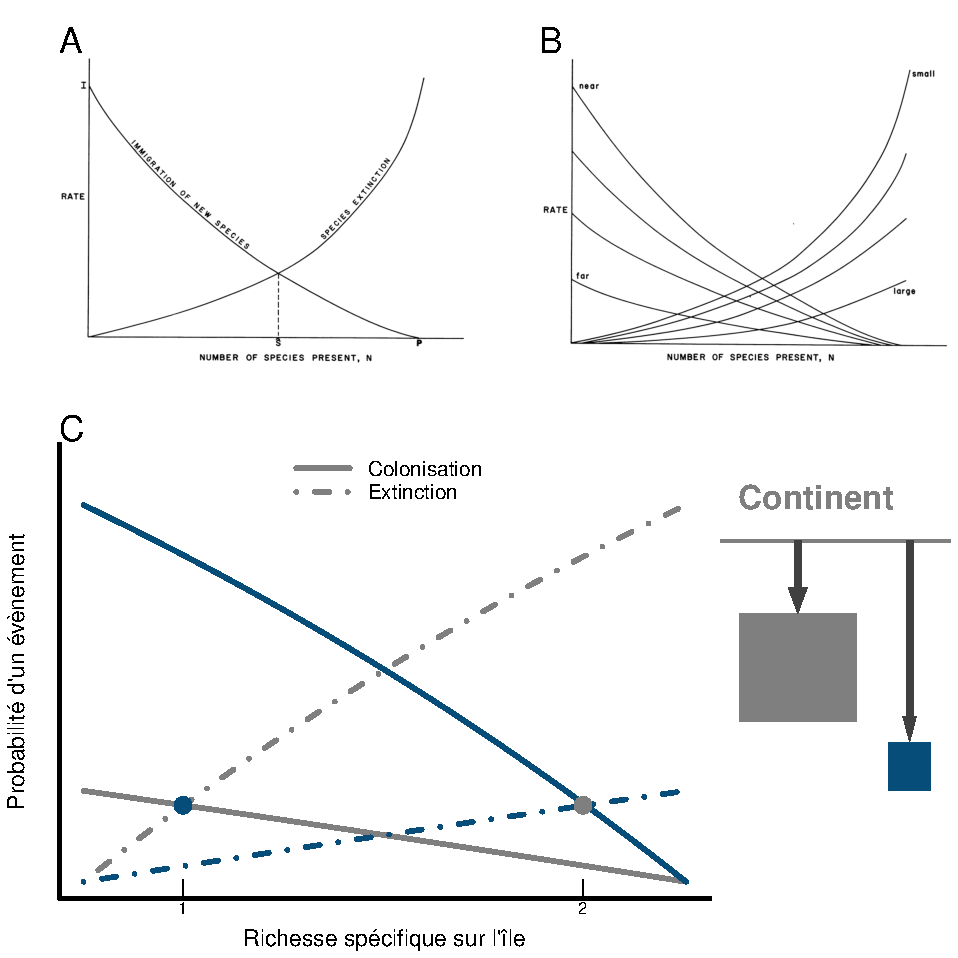
\includegraphics[width=0.90000\textwidth]{fig/fig1.pdf}
\caption[La Théorie de la Biogéographie des Iles (TIB)]{\textbf{La Théorie de la Biogéographie des Iles (TIB)} (A)
illustre l'évolution des taux de colonisation et d'extinction pour deux
îles aux caractéristiques différentes. Les tailles relatives des îles et
les distances qui les séparent du continent sont schématisées sur la
droite, les couleurs associent les îles à leurs courbes respectives. Le
réservoir d'espèce régional (\(P\)) est constitué de 100 espèces, les
taux de colonisation et d'extinction sont exprimés en terme de
probabilité d'événement (de colonisation ou d'extinction). Les points
marquent les intersections entre les courbes d'extinction et de
colonisation c'est-à-dire lorsque ces processus s'équilibrent.
L'abscisse de ces points indique les richesses spécifiques de l'île à
l'équilibre \(S_{eq}\). (B) et (C) sont respectivement les Figures 4 et
5 extraites de l'article de 1963 de MacArthur et Wilson qui livre
essentiellement le même message que celui illustré en (A)
\citep{MacArthur1963}. La forme convexe des courbes de 1963 est
justifiée par des facteurs biologiques qui ne sont pas intégrés dans
l'équation \label{eqMW} qui confère une forme concave aux courbes, comme
montré en (A).\label{fig:figMW}}
\end{figure}

\subsection*{L'importance de la TIB dans des développements théoriques
plus
récents}\label{limportance-de-la-tib-dans-des-duxe9veloppements-thuxe9oriques-plus-ruxe9cents}
\addcontentsline{toc}{subsection}{L'importance de la TIB dans des
développements théoriques plus récents}

\subsubsection*{La théorie des
métapopulations}\label{la-thuxe9orie-des-muxe9tapopulations}
\addcontentsline{toc}{subsubsection}{La théorie des métapopulations}

Bien que ne représentant que cinq pour-cents des terres émergées, ce
sont bien les observations de la faune des îles qui ont mené à une
vision paradigmatique de la biogéographie \citep{Simberloff1974a}.
L'importance des îles s'explique par leur relative abondance, leur
disparité, leur diversité, la relative simplicité des assemblages
biologiques qu'on y trouve et, comme je l'ai évoqué précédemment, la
clarté des flux de migration \citep{Simberloff1974a}. Cette dernière
propriété est souvent absente pour des populations
continentales\footnote{Les îles sont cependant souvent dans des
  archipels où la lecture de ces flux n'est pas si simple.}. La théorie
des métapopulations s'intéresse justement aux populations reliées entre
elles par des flux de migrations \citep{Hanski2010}. Le premier modèle
de métapopulations a été proposé par Levins\footnote{Richard Levins qui
  avec Heatwole est un des co-découvreurs des idées de la TIB.} lors
d'une réflexion sur le contrôle démographique des ravageurs de cultures
\citep{Levins1969}. Pour un ravageur donné, les îlots de culture sont
autant de patchs où une population peut se maintenir et disperser dans
les autres patchs alentours. Levins montre alors que les mesures de la
lutte biologique doivent être conduites à large échelle pour en
augmenter les probabilités de succès, c'est-à-dire d'extinction
régionale du ravageur~\citep{Levins1969}. Le modèle est simple et très
proche de celui de la TIB~: l'évolution de la proportion \(p\) est aussi
gouvernée par des événements de colonisation \(c\) et d'extinction
\(e\)~:

\begin{eqnarray}
\label{eqMW}
\frac{dp}{dt} = cp(1-p)-ep
\end{eqnarray}

La différence fondamentale avec la TIB est que la migration dépend de la
proportion de patchs occupés~: plus elle est importante plus la
migration est importante. Parmi les démonstrations existantes, figurent
les travaux menés par Ikkha Hanski sur les populations du mélitée du
plantain (\emph{Melitaea cinxia}) au sud-ouest de la Finlande
\citep{Hanski1998}. En plus de donner un cadre de pensée plus réaliste
en termes de configuration spatiale, les dynamiques populationnelles
associées sont bien comprises et mènent à des risques d'extinction mieux
évalués \citep{Hanski1998}. C'est aussi un cadre approprié pour insérer
l'étude des flux génétiques liés à l'arrangement spatial des
populations. Ainsi, toujours sur ces mêmes populations de papillon, Ilik
Saccheri et ses collègues montrent qu'en ajoutant le degré
d'hétérozygotie, ils obtiennent des prédictions précises quant à
l'extinction locale des populations \citep{Saccheri1998}. Les travaux
théoriques autour du concept de métapopulations proposent un certain
nombre de paradigmes qui permettent d'évaluer le rôle que jouent les
processus de colonisation et d'extinction dans les variations
spatio-temporelles de la démographie d'une espèce et a été étendu à
l'échelle de la communauté, on parle alors de métacommunauté
\citep{Leibold2004, Holyoak2005}. La prépondérance de ces mécanismes qui
font la force de la TIB et de la théorie des métapopulations a été
poussée à son paroxysme dans la théorie neutre de la biogéographie.

\subsubsection*{La théorie neutre de la biogéographie et le débat
qu'elle
soulève}\label{la-thuxe9orie-neutre-de-la-bioguxe9ographie-et-le-duxe9bat-quelle-souluxe8ve}
\addcontentsline{toc}{subsubsection}{La théorie neutre de la
biogéographie et le débat qu'elle soulève}

La théorie neutre postule l'équivalence écologique entre les différents
individus d'espèces éventuellement différentes et décrit les dynamiques
populationnelles reposant sur les différences d'abondances relatives à
l'échelle régionale et locale. Ainsi, en 1997, dans l'article fondateur
de la théorie neutre, Stephen Hubbell décrit un modèle dans lequel le
remplacement d'un individu mort dans une communauté locale est le
résultat d'un tirage aléatoire~: le nouvel individu peut être soit
recruté localement et la probabilité que l'individu soit d'une espèce
donnée dépend de l'abondance relative de cette dernière dans la
communauté locale, soit le nouvel individu peut-être un immigrant dont
l'identité de l'espèce à laquelle il appartient est liée à l'abondance à
l'échelle régionale de celle-ci \citep{Hubbell1997}. En plus des
exemples donnés dans l'article de 1997, Hubbell montre de manière
convaincante que dans la forêt tropicale du Panama, à la suite d'un
chablis, le recrutement de l'arbre n'est pas prévisible par ces
caractéristiques et que le recrutement est similaire à la composition
des alentours \citep{Hubbell1999}. La dynamique engendrée est appelée la
dérive écologique, et est dominée par la stochasticité qui conduit
presque certainement à l'extinction de toutes les espèces sauf une,
phénomène contrebalancée par l'apparition d'espèces nouvelles
\citep{Hubbell2010, Ricklefs2003}.

La théorie neutre partage beaucoup de caractéristiques avec la TIB~: les
mécanismes fondamentaux sont l'extinction et la colonisation,
l'hypothèse d'équivalence écologique et l'imbrication des échelles
régionales et locales. Comme le fait remarquer Hubbell en 2010 dans le
chapitre qu'il écrit dans \emph{The Theory of Island Biogeography
Revisited}, la théorie neutre place l'équivalence écologique au niveau
des individus et non plus au niveau des espèces \citep{Hubbell2010}. Une
conséquence directe revendiquée par Hubbell est que cette hypothèse est
cohérente avec la forme convexe des courbes de colonisation et
d'extinction décrites par MacArthur et Wilson (voir la figure
\ref{fig:figMW}) qui n'est en fait pas expliquée pas leur modèle
\citep{Hubbell2010}. Le principe d'équivalence et la place importante
que prend le hasard dans cette théorie a soulevé de très vif débats et
donné lieu à des argumentations à charge contre la véracité de cette
théorie \citep[voir par exemple][]{McGill2003, Ricklefs2003}.
L'équivalence écologique doit, à mon sens, être comprise comme une
abstraction de la singularité des espèces, une simplification de la
diversité des systèmes biologiques, nécessaire à l'isolation d'une
portion restreinte des phénomènes en cause dans la répartition
géographique des espèces pour en évaluer le pouvoir explicatif. Bien
qu'un certain nombre de cas d'études permettent de rejeter cette théorie
\citep{McGill2003, John2007}, les défenseurs de la théorie neutre
affirment qu'elle est tout aussi utile quand une étude en démontre la
fausseté \citep{Rosindell2012}. La théorie neutre peut en effet être
présentée comme une jauge qui mesure l'importance des processus de
différentiation de niches \citep{Wennekes2012}. Ainsi, pour certaines
communautés, la dérive écologique est plus importante que pour d'autres,
ce qui été formalisé au travers de travaux théoriques proposant un
continuum de la théorie neutre vers la théorie de la niche écologique
\citep{Gravel2006a}. Malgré les possibilités offertes par ces deux
théories, elles occultent largement les interactions écologiques qui
sont factuelles; si les observations donnent du crédit à ces théories,
une théorie intégrative de la biogéographie doit expliquer pourquoi.

\section*{Le rôle des interactions dans la distribution des
espèces}\label{le-ruxf4le-des-interactions-dans-la-distribution-des-espuxe8ces}
\addcontentsline{toc}{section}{Le rôle des interactions dans la
distribution des espèces}

La thèse que je présente ici a pour objectif de trouver des pistes pour
intégrer les interactions écologiques dans la TIB. Plus précisément, je
souhaite contribuer à i) la compréhension du rôle des interactions
écologiques dans la géométrie de la répartition géographique des
espèces, et ii) la recherche des traces qu'elles pourraient
éventuellement laisser dans les données d'occurrence des espèces. Comme
je l'ai mentionné plus haut cette idée est très ancienne, Wallace le
remarque ainsi ~: «Both competition and predation appear now to be much
more important in biogeography than people had formely guessed» \citep[
p.28]{wallace1881island}.

Le problème de ces relations écologiques est leur spécificité, l'unicité
de chacune d'entre elles, dont découlent un certain nombre de
difficultés pour généraliser. Néanmoins des travaux récents explorent
des pistes prometteuses pour prédire les interactions, notamment sur la
base de relations allométriques entre proie et prédateur
\citep{Gravel2013}. Du point de vue théorique et à l'examen des
chapitres du dernier livre de MacArthur
\citep{macarthur1972geographical}, il apparait que l'intégration des
interactions est une étape clef pour aller vers une biogéographie
intégrative et c'est dans cette direction que j'ai mené ma thèse,
essayant d'apporter des prémices de réponses pour arriver à une telle
synthèse.

\subsection*{Importance des interactions dans la
distribution}\label{importance-des-interactions-dans-la-distribution}
\addcontentsline{toc}{subsection}{Importance des interactions dans la
distribution}

Dans la TIB, les interactions sont en fait omniprésentes en tant qu'une
des composantes principales du processus d'extinction. Cependant, dans
la formulation du modèle, elles ne sont jamais mentionnées
explicitement, cachées dans le taux d'extinction \(e\). Comme je le
montre sur la figure \ref{fig:figMW}, la différence dans l'allure des
courbes dessinées par MacArthur et Wilson et celles obtenues en
supposant un taux d'immigration et de colonisation sont différentes.
D'après les auteurs, l'immigration devient plus difficile lorsque les
espèces s'accumulent sur l'île et les extinctions sont de plus en plus
fréquentes dues à l'intensification des interactions. Pour parler en
termes de réseaux d'interactions, l'accumulation d'espèces sur l'île
sature le réseau local et rend difficile l'intégration d'une nouvelle
espèce qui le rend par ailleurs de plus en plus instable. Une
interprétation communauté-centrée de la TIB est tout à fait possible
mais les liens entre les espèces ne sont pas formulés mathématiquement
en 1967.

Depuis les années 60, la littérature théorique n'a cessé de discuter le
rôle joué par les interactions intra- et inter-spécifiques dans la
distribution spatiale des espèces. Il est reconnu que l'interdépendance
des espèces détermine le caractère favorable de l'environnement au sens
large (biotique et abiotique). En 2009, Robert Holt et Michael Barfield
discutent de l'impact de la prédation sur la répartition d'espèces en
compétition insistant alors sur le rôle majeur des interactions dans le
dessin des aires de répartition \citep{Holt2009}. En 2012, William
Godsoe et Luke H. Harmon introduisent les interactions dans un modèle
simple de distribution d'espèce et montrent comment la probabilité de
présence d'une espèce peut être affectée par la distribution d'une
seconde et concluent alors que cela doit affecter vraisemblablement la
qualité de prédictions des SDMs \citep{Godsoe2012}. La remise en cause
des SDMs se concentrant sur les variables abiotiques est une étape
fondamentale car leur succès depuis la fin du siècle dernier a relégué
les interactions écologiques au second plan en démontrant que la
corrélation avec les variables climatiques étaient peut-être suffisante,
au moins en première approximation pour expliquer les aires de
répartition \citep{Pearson2003}. Pourtant, dès 1998, le travail
précurseur d'Andrew Davis et ses collègues \citep{Davis1998} avait
fortement remis en question l'hypothèse d'indépendance des espèces
\citep{Jeschke2008}. L'expérience, dont les résultats ont été publiés en
1998, est une analyse d'abondance de trois espèces de drosophile le long
d'un gradient de température. Les comparaisons d'abondance sont menées
pour toutes les combinaisons possibles de ces trois mouches (assemblages
à 1, 2 ou 3 espèces) mais aussi en présence ou en absence d'un
parasitoïdes. La démonstration est sans appel~: la compétition et le
parasitisme affectent drastiquement la survie le long du gradient de
température, les interactions écologiques affectant donc très
probablement les réponses aux changements climatiques.

Plus récemment, on constate une large engouement pour intégrer les
relations écologiques dans les modèles de distribution d'espèces
\citep{Kissling2012, Guisan2011}. Ainsi, des modèles de distributions
jointes d'espèces (JSDMs, \emph{Joint Species Distribution Models}) ont
vu le jour dans les dernières années avec comme atout principal la prise
en compte des corrélations entre les occurrences de différentes espèces
\citep{Pollock2014, Ovaskainen2010}. Néanmoins, ces efforts se heurtent
à un manque de maturité des modèles et théories qui cherchent à
rassembler distribution et interactions. Parmi les travaux récents,
Franck Jabot et Jordi Bascompte ont rassemblé métacommunauté et écologie
des réseaux pour souligner l'importance des relations écologiques dans
la répartition géographique des espèces \citep{Jabot2012}. De même,
Dominique Gravel et ses collègues ont introduit en 2011
l'interdépendance proie-prédateur dans le modèle de la TIB menant aux
prémices d'une théorie trophique de la biogéographie des îles
\citep{Gravel2011} préfigurée par Holt \citep{Holt2009a}. Ces travaux
tentent de dépasser l'hypothèse d'équivalence écologique en vue de faire
des prédictions plus précises concernant les compositions spécifiques
attendues localement.

C'est dans la lignée de ces développements théoriques récents que
s'inscrit mon premier chapitre de thèse. J'y montre comment
l'intégration du concept de réseau écologique dans la TIB était possible
tout en ajoutant la reconnaissance de performances plus ou moins
importantes des espèces dans un contexte abiotique donné (niche
écologique). Pour y arriver, je souligne l'intérêt de considérer les
espèces sous la forme d'assemblage plutôt que une à une. Grâce à
l'utilisation de probabilités conditionnelles d'assemblage dans un
environnement abiotique donné, j'explore les conséquences simultanées
des contraintes biotiques et abiotiques sur la distribution d'espèce
(voir la figure \ref{fig:figGTIB} pour une représentation schématique du
modèle). Du point de vue technique, mon travail montre aussi qu'un
retour aux processus stochastiques tels que ceux présentés en 1967 est
une démarche puissante pour ajouter de nouveaux mécanismes dans la TIB.

\begin{figure}
\centering
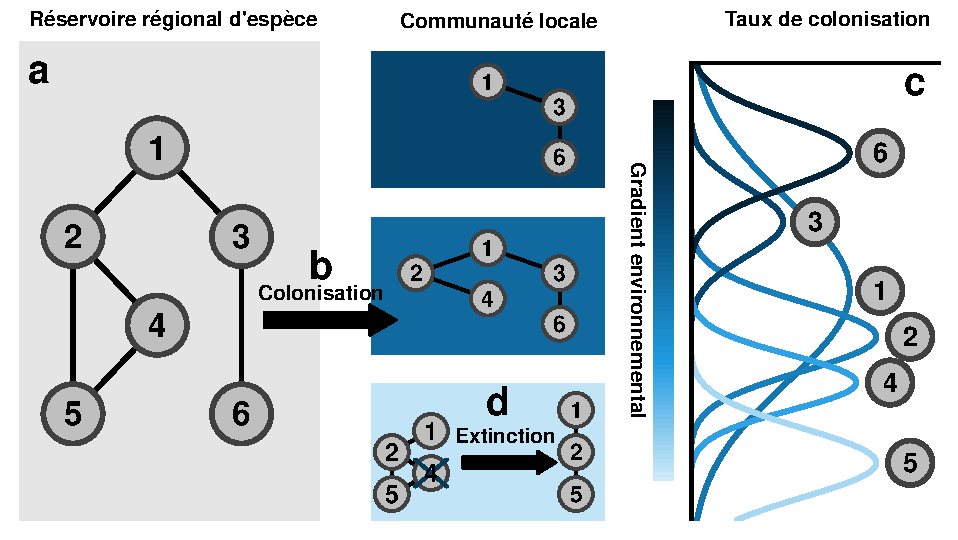
\includegraphics{fig/fig2.pdf}
\caption[Intégration des interactions et des contraintes abiotiques dans la TIB.]{\textbf{Intégration des interactions et des contraintes
abiotiques dans la TIB.} Pour intégrer les interactions j'ai considéré
non pas un ensemble d'espèces indépendantes mais des espèces au sein
d'un réseau décrit à l'échelle régionale (a). Comme dans la TIB, ces
espèces peuvent coloniser l'île (b), mais les taux de colonisation
varient le long d'un gradient environnemental (c). Enfin, les
interactions influencent les taux d'extinction locale (d). Voir le
chapitre \ref{chap1} pour une description complète du
modèle.\label{fig:figGTIB}}
\end{figure}

\subsection*{Un problème d'échelle?}\label{un-probluxe8me-duxe9chelle}
\addcontentsline{toc}{subsection}{Un problème d'échelle?}

En repartant de l'exemple classique de la ségrégation spatiale des
tamias \emph{Eutamias dorsalis} et \emph{E. umbrinus} \citep{Brown1971},
j'ai précédemment mis en évidence qu'une information sur les
interactions est contenue dans les aires de répartition de ces espèces.
Il y a cependant deux caractéristiques qui peuvent conduire à la rareté
de ce type de lecture~: la singularité de l'interaction et son caractère
local. Je reviens un peu plus bas sur la première propriété et m'arrête
ici sur la seconde. Une idée dominante en biogéographie est que les
interactions ont des rôles majeurs à l'échelle locale mais que leurs
conséquences sont de moins en moins perceptible à mesure que l'on
considère des échelles spatiales de plus en plus grandes \citep[voir
l'unique figure de][]{McGill2010}. Du point de vue théorique, c'est tout
à fait ce qui est décrit dans la TIB, car c'est à l'échelle locale que
les interactions influencent l'extinction. Néanmoins, ces conséquences
locales sont présentes sur l'ensemble de la distribution de l'espèce, il
est alors pertinent de se demander pourquoi nous ne sommes pas capables
de détecter les interactions en examinant les distributions d'espèces.
En réalité, bien que cela soit rare, nous avons des preuves que cela
soit possible dans certains cas. En 2010, Nicholas Gotelli et ses
collègues divisent l'avifaune danoise en différentes catégories fondées
sur la similarité écologique et démontrent que les répartitions des
espèces d'une même catégorie se chevauchent moins qu'attendues
aléatoirement \citep{Gotelli2010}. De même, en 2007, Risto Heikkinen et
ses collègues ont obtenu des performances accrues de leurs modèles
statistiques par l'utilisation de la répartition de six espèces de pics
pour expliquer la présence de quatre espèces de hiboux
\citep{Heikkinen2007}. Dans cette même étude, le signal est plus fort
lorsque les données sont dérivées de grilles spatiales à plus petites
mailles (10x10 km contre 40x40 km), ce qui constitue un argument en
faveur d'une dépendance à l'échelle, récemment supportée par d'autres
travaux \citep{Belmaker2015}. Ce qui est remarquable dans les travaux de
Gotelli et de Heikkinen est que l'utilisation de connaissances
biologiques et écologiques a révélé une trace des interactions dans la
distribution des espèces.

La dépendance spatiale de la détection des interactions est facile à
comprendre~: en examinant des données de présence à des échelles
spatiales de plus en plus larges, le nombre d'espèces s'accumule (c'est
le principe de la relation aire-espèce) menant à la dégradation de
l'information potentielle. Cela signifie que l'information nécessaire
pour déceler des empreintes laissées par les interactions sera fournie
par des données à des échelles relativement fines. Cependant, cela ne
permettra pas de conclure sur le rayon d'action de ces interactions.
Pour dépasser la question spatiale, il faut aussi envisager l'impact de
la nature des interactions sur la répartition géographique. Ainsi, en
2014, Miguel Araújo et Alejandro Rozenfeld ont prouvé théoriquement que
les interactions positives (mutualisme) se propageaient davantage que
les interactions négatives \citep{Araujo2014}. Par conséquent, la nature
de la relation qui unit des espèces peut influencer la perte
d'information contenue dans les aires de répartition. Suite à mes
travaux sur l'intégration des interactions, je me suis penché sur un
autre aspect qui peut influencer la perte d'information dans les données
de présence~: l'abondance des interactions. Au chapitre \ref{chap2}, je
montre que les interactions directes et indirectes affectent les données
de distributions mais aussi que l'abondance des interactions rend
difficile de distinguer un quelconque signal~: nous ne sommes plus en
mesure de dire s'il y a des différences entre les paires d'espèces qui
interagissent et celles qui n'interagissent pas. Ce qui est encore plus
intéressant, c'est que j'ai accumulé un certain nombre d'indices dans
des données de présence et d'absence réelle qui semblent confirmer nos
prédictions. Je discute de ces résultats dans le chapitre \ref{chap3} de
cette thèse.

En constatant que l'abondance des interactions peut justifier
l'hypothèse d'indépendance des espèces, je soulève le même paradoxe que
celui relevé par MacArthur dans son œuvre de 1972
\citep{macarthur1972geographical} :

\begin{quote}
A few decades ago it was fashionable for ecologists to study communities
in the arctic on the grounds that these would be very simple communities
and hence easy to understand. Many excellent ecologists still follow
this belief, but there are others who feel that it may be easier to
understand the extremely complex communities of the tropics. This sounds
paradoxical: How can a more complex communities by easier to understand?
A possible answer might be that the complex community has strong
interactions among species so that the lives of the separate species are
less independent than in a simple community. Where there is greater
interdependence, patterns may be more conspicuous.
\end{quote}

Dans cet extrait, MacArthur suggère que la connectance du réseau (le
nombre de lien entre espèces rapporté au nombre de liens possibles) est
vraisemblablement une propriété importante pour comprendre la
répartition des espèces. Peut-être qu'une biogéographie des réseaux
serait une alternative porteuse de généralisations plus accessibles. Un
nouveau problème d'échelle est soulevé, l'échelle biologique appropriée
pour investiguer la répartition géographique des espèces: individus,
population, communauté ou même réseau énergétique?

\subsection*{Vers une biogéographie
énergétique}\label{vers-une-bioguxe9ographie-uxe9nerguxe9tique}
\addcontentsline{toc}{subsection}{Vers une biogéographie énergétique}

Le problème d'échelle biologique est aussi un problème de catégorisation
des espèces. J'ai suggéré que les prédictions étaient plus faciles pour
des espèces généralistes que pour des espèces spécialistes.
Malheureusement, le spectre est très large et plutôt balancé avec un
continuum entre des espèces hyper-spécialistes de d'autres très
généralistes \citep{Poisot2015c}. On peut néanmoins espérer que la
réduction des espèces à un certain nombre de traits
\citep{McGill2006, Poisot2015} doublée d'une réduction des réseaux à un
nombre raisonnable de propriétés puissent permettre des généralisations
utiles dans notre compréhension de la distribution des communautés. Il
m'apparaît aujourd'hui important que le bon niveau de détails dans nos
descriptions des systèmes écologiques quand il est question de prédire
les futures aires de répartitions des espèces.

Une piste prometteuse pour prolonger la recherche des propriétés est, me
semble-t-il, de s'appuyer sur la nature profonde des espèces~: des
systèmes énergétiques qui se perpétuent. La lecture de la théorie de la
dynamique du budget énergétique de Sebastian A. L. M. Kooijman
\citep{Kooijman2000a} m'a été très profitable pour cerner les
possibilités offertes par une telle approche. S'il est possible, comme
le suggèrent les travaux de Kooijman, de dériver de manière précise un
grand nombre de propriétés énergétiques des espèces sur leur masse et
leur forme, alors les espoirs sont grands de pouvoir trouver des règles
d'assemblages fiables des communautés et donc de comprendre d'un point
de vue mécanistique les extinctions locales. Ce sont les mêmes espoirs
que ceux nourrit par la théorie métabolique de l'écologie qui rassemble
des relations entre la taille des espèces, différentes de leurs
propriétés \citep{Brown2004} qui montrent en somme qu'il est possible
d'aller au-delà de l'espèce \citep{Poisot2015}. Mes réflexions sur
l'intersection entre la TIB et une vision énergétique de l'écologie sont
présentées au chapitre \ref{chap4} de la présente thèse. Dans ce
chapitre, j'explique en quoi l'approche énergétique est pertinente pour
intégrer des interactions et les contraintes données par un flux
énergétique fini. Je propose des pistes pour lever des difficultés
posées par le calcul précis de la consommation de chaque niveau
trophique et montre ce qu'apporte l'idée que les écosystèmes sont
énergétiquement saturés. Ce chapitre est également une ouverture vers
les projets de recherche que je souhaiterais mener dans un futur proche.
